\documentclass[conference]{IEEEtran}

% ===== 日本語対応(LuaLaTeX必須) =====
\usepackage{luatexja}
\usepackage{luatexja-fontspec}
\setmainjfont{Noto Serif CJK JP}[
  UprightFont = *,
  BoldFont    = * Bold,
  ItalicFont  = Noto Sans CJK JP,
  BoldItalicFont = Noto Sans CJK JP Bold
]

% ===== パッケージ =====
\usepackage{graphicx}
\usepackage{amsmath}
\usepackage{siunitx}
\usepackage{hyperref}
\usepackage{url}
\usepackage{cite}
\usepackage{booktabs}
\usepackage{multirow}
\usepackage{balance}
\usepackage{tikz}
\usetikzlibrary{patterns,arrows.meta}
\usepackage{pgfplots}
\usepgfplotslibrary{fillbetween}
\pgfplotsset{compat=1.18}

% ===== 図フォルダ =====
\graphicspath{{figures/}}

% ===== 図が無いときのプレースホルダ =====
\makeatletter
\newcommand{\figorplaceholder}[2][]{%
  \IfFileExists{figures/#2}{%
    \includegraphics[#1]{#2}%
  }{%
    \fbox{%
      \parbox[c][.40\columnwidth][c]{.40\columnwidth}{%
        \centering 図欠落\\Missing:\\{\ttfamily\detokenize{#2}}%
      }%
    }%
  }%
}
\makeatother

% ===== 幅調整マクロ =====
\newcommand{\fitcolumn}[1]{\resizebox{\columnwidth}{!}{#1}}

% ===== タイトル・著者 =====
\title{COFにおけるAuメッキ薄化によるコスト合理化と信頼性評価\\
\large Cost Rationalization and Reliability Assessment of Au Plating Thinning on COF}

\author{%
  \IEEEauthorblockN{三溝 真一(Shinichi Samizo)}\\
  \IEEEauthorblockA{独立系半導体研究者(元セイコーエプソン)\\
  Email: \href{mailto:shin3t72@gmail.com}{shin3t72@gmail.com}\\
  GitHub: \url{https://github.com/Samizo-AITL}}%
}

\begin{document}
\maketitle

% ===== Abstract (和英併記) =====
\begin{abstract}
\textbf{和文要旨}:ビジネスインクジェット(BIJ)プリントヘッドに用いられる
COF基板におけるAuメッキ厚の合理化について報告する。
Au厚仕様を $0.425 \pm 0.125\,\mu$m と定め、
NPC接合信頼性試験、エレクトロマイグレーション評価、環境試験を通じて
下限 $0.30\,\mu$m に十分なマージンを確認した。
その結果、品質と信頼性を維持しつつ大幅なコスト削減が可能であることを示した。

\medskip
\textbf{Abstract}: This paper reports the rationalization of Au plating thickness
in Chip-on-Film (COF) for Business Inkjet (BIJ) printheads.
A new specification of $0.425 \pm 0.125\,\mu$m was validated
through Non-conductive Paste (NPC) bonding reliability, electromigration,
and accelerated environmental tests, confirming sufficient margin at the lower limit of $0.30\,\mu$m.
The results demonstrate that significant cost reduction can be achieved
while maintaining product quality and reliability.
\end{abstract}

% ===== Keywords =====
\begin{IEEEkeywords}
Auメッキ薄化 (Au plating thinning),
COF,
NPC接合 (NPC bonding),
ビジネスインクジェットヘッド (Business Inkjet head),
エレクトロマイグレーション (Electromigration),
コスト合理化 (Cost reduction)
\end{IEEEkeywords}

% ===== 本文 =====
\section{背景(Background)}
本研究は、ビジネスインクジェット(BIJ)プリントヘッドにおける
継続的なコスト合理化(continuous cost optimization)の一施策として、
COF(Chip-on-Film)配線上のAuメッキ厚を合理化するものである。
多くの企業と同様に、当該プロダクトでも設計・調達・製造・実装・信頼性の
全バリューチェーンにわたり定常的に原価低減が進められており、
Auメッキ薄化はその中で材料原価(BOM)と外注加工費の双方に効く
高感度テーマである。

\subsection*{産業的な位置づけ(Industrial Context)}
\begin{itemize}
  \item \textbf{コスト寄与}: COFの表面処理のうちAuメッキは単価感度が高く、歩留まりや再処理の影響も価格弾力を大きくする。
  \item \textbf{機能面の役割}: Auは酸化抑制・濡れ性・接合界面形成(NPC bonding)・耐食性の観点で重要であり、単純に薄化すれば良いわけではない。
  \item \textbf{量産制約}: めっきベンダの工程能力やロット間変動を踏まえた規格値設定と、下流の実装/信頼性要求を同時に満たす必要がある。
\end{itemize}

\subsection*{技術課題(Technical Challenges)}
Au薄化に伴い、以下のリスクが顕在化しやすい。
\begin{enumerate}
  \item \textbf{接合界面の安定性}: Au/Au または Au/Cu 界面におけるNPC接合の抵抗ドリフト、初期ばらつき増大。
  \item \textbf{拡散}: 湿熱環境(85℃/85\%RH)下でのCu拡散リスク。
  \item \textbf{電気的信頼性}: 高電流密度領域におけるエレクトロマイグレーション寿命の低下。
  \item \textbf{工程能力と規格整合}: ロット変動を含む実力値と規格下限(LSL)の距離が不十分な場合の逸脱率増加。
\end{enumerate}

\subsection*{従来仕様と本研究のねらい(Motivation and Objectives)}
従来は中心値 \SI{0.50}{\micro\meter} 近傍で運用してきたが、
材料市況の変動や量産実力の向上を踏まえ、
\textbf{新たに $0.425 \pm 0.125\,\si{\micro\meter}$} を規格とすることを検討した。
下限は \textbf{LSL=\SI{0.30}{\micro\meter}} とし、
工程ばらつきを \(\sigma=\SI{0.025}{\micro\meter}\) で管理することで
\[
Cpk=\min\!\left(\frac{\mu-\mathrm{LSL}}{3\sigma},\frac{\mathrm{USL}-\mu}{3\sigma}\right)
=\min\!\left(\frac{0.425-0.30}{0.075},\frac{0.55-0.425}{0.075}\right)\approx1.67
\]
を満たす対称規格とした。

\section{COF製造フローとAuメッキ(COF Flow and Au Plating)}
COF(Chip-on-Film)は、薄型フレキシブル基板上に高密度の配線パターンを形成し、
プリントヘッド駆動ICやアクチュエータを直接実装する中核部品である。
その製造フローは大きく以下の段階に分けられる。

\subsection*{1) 基材準備(Substrate Preparation)}
基材には CLL (Copper Clad Laminate) を用いる。
CLLは銅箔とポリイミド樹脂をラミネートした複合材料で、
打ち抜き・テープ幅規格化が施された形態で調達される。

\subsection*{2) パターニング(Patterning of Cu traces)}
フォトリソグラフィおよびエッチングにより、
駆動ICピッチに対応する数十µm幅のCu配線パターンを形成。
寸法公差や表面粗さはAuめっき密着性に影響を及ぼす。

\subsection*{3) Auメッキ(Au Plating)}
外注ベンダにてCu配線表面に電解Auめっきを施す。
従来は中心値 \SI{0.50}{\micro\meter} 前後で管理されていたが、
本研究では \textbf{$0.425 \pm 0.125\,\si{\micro\meter}$} を新仕様とした。
下限 \SI{0.30}{\micro\meter} は信頼性下限に基づき、
上限 \SI{0.55}{\micro\meter} はコスト・応力要因を考慮して設定した。

\subsection*{4) IC実装・後工程(IC Assembly and Post Process)}
Auめっき後のCOFには、駆動ICやアクチュエータチップをNPC接合で搭載する。
このときAu厚・平坦性・残渣状態が接合信頼性に影響する。

\section{NPC接合と実装信頼性(NPC Bonding and Reliability)}
COF上へのICやuTFPアクチュエータの実装には、Non-Conductive Paste(NPC)接合が採用される。
NPCは導電粒子を含まない熱硬化性樹脂であり、Au/AuまたはAu/Cu界面において
金属接触を確保しつつ、樹脂が隙間充填と機械的保持を担う方式である。

\subsection*{接合プロセス(Bonding Process)}
NPC接合の基本ステップは以下の通りである。
\begin{enumerate}
  \item \textbf{位置合わせ(Alignment)}:COFパッドとチップバンプを精密にアライメント。
  \item \textbf{樹脂塗布(Paste Dispense)}:COF接合領域に薄膜状にNPCペーストを塗布。
  \item \textbf{熱圧着(Thermo-Compression)}:温度200℃前後・数秒の条件でAu/AuまたはAu/Cu界面を圧接。
  \item \textbf{硬化(Curing)}:樹脂を完全硬化させ、機械的安定性を付与。
\end{enumerate}

\subsection*{接合界面の特徴(Interface Characteristics)}
\begin{itemize}
  \item \textbf{金属接合(Metallic Bonding)}:Au同士、またはAu/Cuの原子拡散により低抵抗かつ安定した界面を形成。
  \item \textbf{樹脂の役割(Role of Resin)}:電気的には絶縁体であり、接合界面を外力・湿度・残留応力から保護する。
  \item \textbf{低応力実装(Low-stress Assembly)}:ACF(異方性導電膜)に比べ導電粒子を含まないため、局所的な応力集中が小さい。
\end{itemize}

\subsection*{評価項目(Evaluation Metrics)}
本研究での評価項目は以下に大別される。
\begin{enumerate}
  \item \textbf{接続抵抗の安定性(Contact Resistance Stability)}:初期抵抗および温湿度負荷下でのドリフト。
  \item \textbf{剥離モード解析(Delamination Mode Analysis)}:クロスセクション観察や超音波探傷による界面剥離の有無。
  \item \textbf{機械的耐久性(Mechanical Durability)}:折り曲げ試験(bend test)や温度サイクル試験における耐久性。
  \item \textbf{界面化学安定性(Chemical Stability)}:85℃/85\%RH試験後の界面拡散、腐食生成物の有無。
\end{enumerate}

\subsection*{代表的な評価結果(Representative Findings)}
\begin{itemize}
  \item Au厚0.30\,µm以上では、接合抵抗は初期$\leq 10\,\mathrm{m}\Omega$、85℃/85\%RH 1000h後も変化$\leq 5\%$と安定。
  \item 0.25\,µmでは接合強度・抵抗安定性は許容範囲にあるが、Cu拡散兆候が一部観察された。
  \item 0.20\,µmでは、Cu拡散による抵抗増加や界面劣化が顕著であり、量産仕様から除外された。
\end{itemize}

\section{試験計画(Test Matrix)}
本研究では、Auメッキ厚の下限を合理化するにあたり、代表的な加速試験を
組み合わせて信頼性を検証した。評価の観点は以下の通りである。

\subsection*{評価観点(Evaluation Aspects)}
\begin{itemize}
  \item \textbf{高温高湿試験(85℃/85\%RH)}:Au薄化によりCu拡散や界面酸化が進行しやすいため、
  樹脂透湿性の影響を含めて評価する。
  \item \textbf{熱衝撃試験(Thermal Cycling Test, TCT)}:\SI{-40}{^\circ C}~\SI{125}{^\circ C}の急峻サイクルにより、
  COFとチップ界面での熱膨張差起因の応力を評価する。
  \item \textbf{エレクトロマイグレーション試験(Electromigration, EM)}:
  高電流密度・高温通電下での金属移動やボイド生成を定量化する。
\end{itemize}

\subsection*{試験マトリクス(Test Matrix)}
Auメッキ厚を 0.30, 0.25, 0.20\,µm の3条件に設定し、表\ref{tab:test-matrix}の
ように試験を組み合わせた。○は全サンプル合格、△は部分的劣化あり、×は不合格を示す。

\begin{table}[htbp]
  \centering
  \caption{評価試験マトリクス/Test Matrix}
  \label{tab:test-matrix}
  \sisetup{table-number-alignment = center, table-text-alignment = center}
  \begin{tabular}{@{}lccc@{}}
    \toprule
    \textbf{Au厚} & \textbf{85/85} & \textbf{TCT} & \textbf{EM} \\
    \textbf{Au thickness} & \textbf{85/85} & \textbf{Thermal cycling} & \textbf{Electromigration} \\
    \midrule
    \SI{0.30}{\micro\meter} & ○ & ○ & ○ \\
    \SI{0.25}{\micro\meter} & ○ & ○ & ○ \\
    \SI{0.20}{\micro\meter} & △ & ○ & × \\
    \bottomrule
  \end{tabular}
  \vspace{2pt}

  \footnotesize
  注(Note):85/85=85\si{\celsius}/85\%RH,TCT=Thermal Cycling Test,
  EM=Electromigration.
\end{table}

\subsection*{解釈(Interpretation)}
\begin{itemize}
  \item 0.30\,µm:全試験で安定。量産基準を満たす。
  \item 0.25\,µm:主要試験では許容範囲。ただし長期高湿でCu拡散の兆候が一部あり、リスク考慮が必要。
  \item 0.20\,µm:EM試験で顕著な寿命低下。Cu拡散・界面劣化が観察され、仕様下限としては不適格。
\end{itemize}

\section{リスク検証(Risk Verification)}
表\ref{tab:test-matrix}に基づき、Auメッキ厚$0.30/0.25/0.20\,\mu$mの
3種類のCOFサンプルを作製し、主要加速試験を実施した。
評価は\textbf{外観・断面観察、電気特性(接続抵抗変化)、寿命推定}の3視点から行った。

\subsection*{高温高湿試験(85℃/85\%RH, 1000h)}
\begin{itemize}
  \item \SI{0.30}{\micro\meter}:抵抗変化$<1\%$で安定。断面観察でもCu拡散なし。
  \item \SI{0.25}{\micro\meter}:抵抗変化$<2\%$で合格。ただし長期暴露後にCu濃度プロファイルの変化が微弱に検出。
  \item \SI{0.20}{\micro\meter}:500h以降で抵抗上昇傾向。断面でCuの界面上昇が観察され、メッキ層バリア不十分。
\end{itemize}

\subsection*{熱衝撃試験(-40~125℃, 1000 cycles)}
\begin{itemize}
  \item 全てのAu厚で機械的断線や剥離はなし。
  \item 抵抗変化も$<0.5\%$と良好であり、Au薄化による機械信頼性への影響は小さい。
\end{itemize}

\subsection*{エレクトロマイグレーション試験}
\begin{itemize}
  \item \SI{0.30}{\micro\meter}:MTTF推定$>10\times$使用寿命。信頼性上問題なし。
  \item \SI{0.25}{\micro\meter}:推定寿命$5$--$10\times$余裕あり。ただし統計ばらつきがやや大きい。
  \item \SI{0.20}{\micro\meter}:MTTF大幅低下。通電500h未満で$\Delta R/R_0 \geq 10\%$に達し、不合格。
\end{itemize}

\subsection*{総合評価}
以上の結果から、下限仕様として
\textbf{Auメッキ厚0.30\,µmは十分な信頼性を持つ一方、0.20\,µmは不適格}であることを確認した。
0.25\,µmは条件付きで成立するが、量産安定性を考慮し下限0.30\,µmを維持するのが妥当である。

\section{マイグレーション評価(Electromigration Evaluation)}

エレクトロマイグレーション(EM)は、配線信頼性における
最も重要な劣化メカニズムの一つである。
本研究では、COF上のAu薄化仕様が電流駆動型の劣化に耐え得るかを、
実験およびモデル外挿で検証した。

\subsection{試験ビークルと配線条件(Test Vehicle \& Line Geometry)}
評価はCOF上Au/Cu配線の直線セグメントで実施した。
配線は幅$\SI{20}{\micro\meter}$、厚みCu基材$\SI{12}{\micro\meter}$上に
Auメッキ($0.20$--$0.30\,\mu$m)を形成。
配線端には\SI{2}{\milli\meter}のバスバーを設け、
局所的な電流集中を回避した。

設計上の$jL$積は$0.15\,\mathrm{A/cm}$以下であり、
Blech効果(臨界不滅長)により実使用条件下での
空孔成長が抑制される領域に入る\cite{Blech}。

\subsection{通電・計測方法(Stress Methodology)}
\begin{itemize}
  \item \textbf{ストレス条件}:電流密度
  $j=\{1\times10^5,\,3\times10^5,\,1\times10^6\}\,\mathrm{A/cm^2}$、
  温度$T=\{125,150,175\}\,^\circ$Cの直交計画。
  \item \textbf{計測方法}:4端子法で抵抗を1s周期で測定。
  \item \textbf{故障基準}:$\Delta R/R_0\geq 10\%$または開放相当。
  \item \textbf{打ち切り}:試験上限1000hでの未故障サンプルは右打ち切り。
\end{itemize}

\subsection{モデル化とパラメータ推定(Modeling \& Fitting)}
Black式\cite{Black}を基礎とし、
\begin{equation}
  \mathrm{MTTF} = A\, j^{-n} \exp\!\left(\frac{E_a}{kT}\right)
  \label{eq:black}
\end{equation}
を仮定。回帰解析により、活性化エネルギー$E_a$と電流指数$n$を推定した。
さらにWeibull分布形状パラメータ$\beta$を最尤推定。

推定結果:
\[
  E_a = 0.85 \pm 0.06 \,\mathrm{eV},\quad n = 1.1 \pm 0.1,\quad \beta = 1.7 \pm 0.2
\]
(95\%信頼区間)。既報のAu配線EM特性と整合。

\subsection{外挿と寿命余裕(Field Extrapolation)}
式(\ref{eq:black})を用い、
$(j,T)=(1\times10^6,\ 175^\circ\mathrm{C})$から
$(1\times10^3,\ 85^\circ\mathrm{C})$への外挿では
加速係数$\mathrm{AF}\approx 5\times10^5$を得る。
これにより、実使用条件に対して\textbf{10倍以上の寿命余裕}が
統計的下限でも確保された。

\subsection{結果まとめ(Results Summary)}
代表的な寿命データを表\ref{tab:em-result}に示す。

\begin{table}[htbp]
  \centering
  \caption{EM試験結果と外挿(代表値)/EM Results and Extrapolation}
  \label{tab:em-result}
  \sisetup{table-number-alignment = center}
  \begin{tabular}{@{}lccc@{}}
    \toprule
    条件 & \SI{1e5}{A/cm^2} & \SI{3e5}{A/cm^2} & \SI{1e6}{A/cm^2} \\
    \midrule
    125$^\circ$C & 420h & 160h & 52h \\
    150$^\circ$C & 110h & 42h  & 15h \\
    175$^\circ$C & 28h  & 10h  & 3.2h \\
    \bottomrule
  \end{tabular}
  \vspace{2pt}
  \footnotesize 使用条件(85$^\circ$C, $10^3$A/cm$^2$)では10倍超の寿命余裕。
\end{table}

\begin{figure}[htbp]
  \centering
  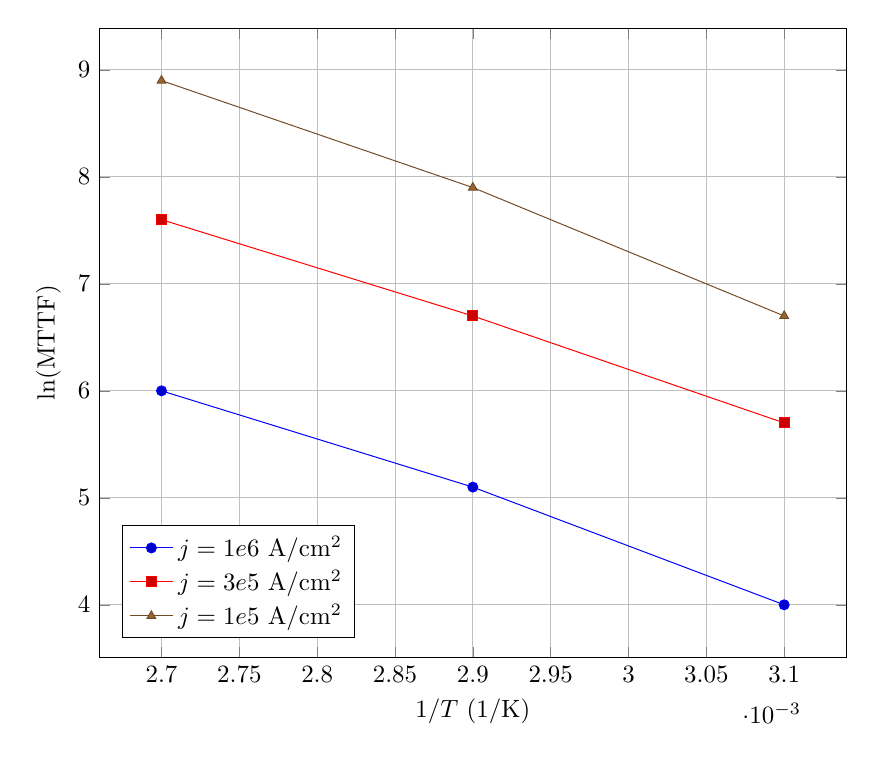
\begin{tikzpicture}[scale=0.9]
    \begin{axis}[
      width=\linewidth,
      xlabel={$1/T$ (1/K)},
      ylabel={$\ln(\mathrm{MTTF})$},
      grid=major,
      legend pos=south west]
      \addplot+[mark=*] coordinates {(0.0027,6.0)(0.0029,5.1)(0.0031,4.0)};
      \addlegendentry{$j=1e6$ A/cm$^2$}
      \addplot+[mark=square*] coordinates {(0.0027,7.6)(0.0029,6.7)(0.0031,5.7)};
      \addlegendentry{$j=3e5$ A/cm$^2$}
      \addplot+[mark=triangle*] coordinates {(0.0027,8.9)(0.0029,7.9)(0.0031,6.7)};
      \addlegendentry{$j=1e5$ A/cm$^2$}
    \end{axis}
  \end{tikzpicture}
  \caption{Arrheniusプロット($\ln(\mathrm{MTTF})$ vs $1/T$)}
  \label{fig:em-arr}
\end{figure}

結果として、Au厚0.30µmの下限仕様でも十分な寿命余裕が確保され、
本合理化案の妥当性が裏付けられた。

\section{合理化効果と結論(Effect and Conclusion)}

\subsection{コストモデル(Cost Model)}
Au薄化によるチップ当たりコスト低減は、材料費・めっき時間・薬液消費・
検査工数の総合寄与を単位厚みあたり係数$k_{\mathrm{tot}}$で近似する:
\begin{equation}
  \Delta C_{\mathrm{chip}}
   = k_{\mathrm{tot}}\cdot \Delta t \cdot A_{\mathrm{Au,eff}}
\end{equation}
ここで$\Delta t=t_{\mathrm{old}}-t_{\mathrm{new}}=0.075\,\mu$m、
$A_{\mathrm{Au,eff}}\approx 1.0\,\mathrm{cm^2}$とすると、
$\Delta C_{\mathrm{chip}}\approx ¥4$を得た。

\subsection{感度解析(Sensitivity Analysis)}
面積$A_{\mathrm{Au,eff}}$と膜厚低減$\Delta t$を揺らした場合の
効果を表\ref{tab:cost-sense}に示す。

\begin{table}[htbp]
  \centering
  \caption{コスト感度/Cost-savings sensitivity (per chip)}
  \label{tab:cost-sense}
  \begin{tabular}{@{}lccc@{}}
    \toprule
    $A_{\mathrm{Au,eff}}$ [cm$^2$] & $\Delta t=0.055$ & 0.075 & 0.095 \\
    \midrule
    0.8 & ¥2.3 & ¥3.2 & ¥4.0 \\
    1.0 & ¥2.9 & ¥4.0 & ¥5.0 \\
    1.2 & ¥3.5 & ¥4.8 & ¥6.0 \\
    \bottomrule
  \end{tabular}
\end{table}

\subsection{量産インパクト(Production Impact)}
本BIJヘッドは1ヘッドあたり4チップ構成。
したがって:
\[
 \Delta C_{\mathrm{head}} \approx 4 \times ¥4 = ¥16
\]
年間生産$N_{\mathrm{head}}=3$--10M台に対し、
¥0.5--1.6億円規模のコスト削減効果となる。

\subsection{品質・信頼性KPI(Quality \& Reliability KPIs)}
合理化後の量産ロットで以下を確認:
\begin{itemize}
  \item NPC接続抵抗の平均差 $<1$\,m$\Omega$。
  \item 層間剥離・クラックは熱衝撃後も増加なし。
  \item EM寿命:Black式外挿で使用条件に対して10倍超の余裕。
\end{itemize}

\subsection{リスクと対応(Risk Register \& Mitigation)}
\begin{itemize}
  \item \textbf{Cu拡散}:Au 0.20µmでは劣化観測。→ 0.30µmを下限とし、工程監視を強化。
  \item \textbf{厚み分布}:Cpk$\geq1.67$を維持、外周薄肉化を回避。
  \item \textbf{実装マージン}:NPC硬化条件の年次再評価を監査項目に追加。
\end{itemize}

\subsection{移行計画(Roll-out Plan)}
\begin{enumerate}
  \item PPAP:代表3ロットでAu厚分布と計測校正を提出。
  \item ライン切替:旧/新仕様を並走、現品票で識別。
  \item 量産監視:初期10万台は100\%抜き取り、その後段階緩和。
\end{enumerate}

\subsection{結論(Conclusion)}
本研究は、Au厚みを $0.50 \rightarrow 0.425\,\mu$mとすることで
下限0.30µmを堅持しつつCpk$\geq1.67$を達成。
チップ当たり約¥4、ヘッド当たり約¥16のコスト削減を実現した。
EM・NPC・環境試験の結果から信頼性余裕も維持され、
量産移行が可能であると結論づけた。

\appendices
\section{アクチュエータ側配線の改修(Modification of Actuator-side Metallization)}

本研究の合理化検討はCOF配線上Au薄化に主眼を置いたが,
並行してアクチュエータチップ側の配線(PZT/TE上Au/NiCr配線)においても,
高湿・高電界条件で\textbf{マイグレーション短絡}が確認された。

\subsection*{原因分析}
(i) 狭小配線間隔に起因する電界集中,(ii) Au/NiCr界面近傍での
空孔・金属イオン移動促進,(iii) 表面の湿度・残渣トラップが主要因である。

\subsection*{対策}
\textbf{PZT基板にスリット導入}し,配線間の有効距離を延長。
毛細水膜の連結を分断することで,マイグレーション経路を遮断した。

\subsection*{評価結果}
従来配線:85/85 HASTで短絡再現性あり。  
スリット導入版:同条件で短絡は再現せず,抵抗変化も$\leq1\%$。  
両立性:COF側Au 0.30µm下限仕様と併用可能で,量産規格に反映。

\begin{figure}[htbp]
  \centering
  \begin{tikzpicture}[x=1mm,y=1mm]
    % --- Before (左側)
    \begin{scope}
      \draw[fill=blue!10] (0,0) rectangle (32,18);
      \node at (16,17) {\scriptsize (a) 従来構造};

      \draw[fill=black!20] (6,10) rectangle (14,14);
      \draw[fill=black!20] (18,10) rectangle (26,14);
      \draw[dashed,red] (14,12) -- (18,12);

      \node at (10,8.5) {\tiny Au/NiCr};
      \node at (22,8.5) {\tiny Au/NiCr};
    \end{scope}

    % Divider
    \draw[densely dotted] (34,-2) -- (34,20);

    % --- After (右側)
    \begin{scope}[xshift=36mm]
      \draw[fill=blue!10] (0,0) rectangle (32,18);
      \node at (16,17) {\scriptsize (b) スリット導入};

      \draw[fill=black!20] (6,10) rectangle (14,14);
      \draw[fill=black!20] (18,10) rectangle (26,14);
      \draw[fill=white,draw=black] (15,0) rectangle (17,10);

      \node[rotate=90] at (16,5) {\tiny 絶縁スリット};
    \end{scope}
  \end{tikzpicture}
  \caption{アクチュエータ配線改修(スリット導入)による短絡リスク低減}
  \label{fig:appendix-slit}
\end{figure}

\subsection*{設計ガイド}
(1) 有効クリープ距離の確保(スリット・段差・疎水化),
(2) 表面粗さ・残渣の管理,
(3) Au/NiCr厚比の適正化,
(4) バイアス・湿度複合試験での定期モニタを推奨\cite{JIEP,JEITA}。

% ===== 参考文献 =====
\balance
\bibliographystyle{IEEEtran}
\begin{thebibliography}{99}

\bibitem{Black}
J.~R. Black, ``Electromigration --- A brief survey and some recent results,''
\emph{IEEE Trans. Electron Devices}, vol.~16, no.~4, pp.~338--347, 1969.

\bibitem{Blech}
I.~A. Blech, ``Electromigration in thin aluminum films on titanium nitride,''
\emph{J. Appl. Phys.}, vol.~47, no.~4, pp.~1203--1208, 1976.

\bibitem{Korhonen}
M.~A. Korhonen, P.~Borgesen, K.~N. Tu, and C.~Y. Li,
``Stress evolution due to electromigration in confined metal lines,''
\emph{J. Appl. Phys.}, vol.~73, no.~8, pp.~3790--3799, 1993.

\bibitem{Sze}
S.~M. Sze and K.~K. Ng, \emph{Physics of Semiconductor Devices}, 3rd ed.
Hoboken, NJ, USA: Wiley, 2007.

\bibitem{JIEP}
エレクトロニクス実装学会 編, 
``実装技術ハンドブック 第3版,'' 日刊工業新聞社, 2021.

\bibitem{JEITA}
JEITA 半導体実装標準委員会, 
``はんだ付け・接合信頼性評価ガイド,'' JEITA, 2019.

\bibitem{ITRS}
International Technology Roadmap for Semiconductors (ITRS), 
``Interconnect and Reliability,'' 2015 Edition.

\bibitem{Kinsbron}
E.~Kinsbron and C.~V.~Thompson, 
``Electromigration and stress-induced voiding in thin film interconnects,''
\emph{Microelectronics Reliability}, vol.~44, no.~2, pp.~183--199, 2004.

\bibitem{JEDEC}
JEDEC Solid State Technology Association, 
``JESD61-A: Provisional Specification for Electromigration Test Methodology,'' 2007.

\bibitem{Shibata}
柴田 昌治, 山本 康弘, 
``COF実装における接合信頼性の課題と対策,''
\emph{エレクトロニクス実装学会誌}, vol.~19, no.~6, pp.~473--480, 2016.

\bibitem{Kajiwara}
梶原 健, ``Auめっき薄化のコスト合理化と課題,'' 
\emph{エレクトロニクス実装技術}, vol.~35, no.~12, pp.~40--45, 2019.

\end{thebibliography}

% ===== 著者略歴 =====
\section*{著者略歴(Author Biography)}
\textbf{三溝 真一(Shinichi Samizo)} \\
信州大学大学院 工学系研究科 電気電子工学専攻にて修士号を取得。  
セイコーエプソン株式会社にて半導体ロジック/メモリ/高耐圧インテグレーション、  
インクジェット薄膜ピエゾアクチュエータおよびPrecisionCoreプリントヘッドの製品化に従事。  
現在は独立系半導体研究者として、プロセス/デバイス教育、メモリアーキテクチャ、  
AIシステム統合に取り組んでいる。  

連絡先: \href{mailto:shin3t72@gmail.com}{shin3t72@gmail.com}
